% -*- TeX:Rnw:si -*-
% ----------------------------------------------------------------
% .R Sweave file  ************************************************
% ----------------------------------------------------------------
%%
%\documentclass[a4paper,12pt,english]{article}
\documentclass[a4paper,12pt,slovene]{article}
\newcommand{\SVNRevision}{$Rev: 4 $}
\newcommand{\SVNDate}{$Date:: 2008-04-22$}
\usepackage{babel}
\input{abpkg}
\input{abcmd}
\input{abpage}
\usepackage{pgf,pgfarrows,pgfnodes,pgfautomata,pgfheaps,pgfshade}
\usepackage{amsmath,amssymb}
\usepackage{colortbl}
\usepackage{Sweave}
\input{mysweave}

%\SweaveOpts{echo=false}
\setkeys{Gin}{width=0.7\textwidth}
\usepackage{lmodern}
\input{abfont}
%\SweaveOpts{keep.source=true}
%\setkeys{Gin}{width=0.8\textwidth} % set graphicx parameter
% ----------------------------------------------------------------
\begin{document}
%% Sweave settings for includegraphics default plot size (Sweave default is 0.8)
%% notice this must be after begin{document}
%%% \setkeys{Gin}{width=0.9\textwidth}
% ----------------------------------------------------------------
\title{Minimumi vsot odklonov in razmerij}
\author{A. Blejec}
%\address{}%
%\email{}%
%
%\thanks{}%
%\subjclass{}%
%\keywords{}%

%\date{}%
%\dedicatory{}%
%\commby{}%
\maketitle
% ----------------------------------------------------------------

% ----------------------------------------------------------------



\section{Vpliv velikih vrednosti na vsote odklonov}

Za prikaz lastnosti vsote absolutnih odklonov od $a$
$$\sum |x-a|$$
vsote kvadratnih odklonov od $a$
$$\sum (x-a)^2$$
in produkta razmerij $x$ in $a$
$$\prod e^{log(x/a)^2}$$
sem pripravil funkcijo \code{showMinDeviation}. Funkcija je v razdelku \ref{s:fct}.

Funkcija prika�e vrednosti odklonov za razli�ne vrenosti $a$, pri �emer se ena od vrednosti medpodatki spreminja od zelo majhne do zelo velike (argument \code{Xs=20}). Pri tem opazimo, da je minimum dose�en pri mediani, povpre�ju (aritmeti�ni sredini) in pri geometrijski sredini.


Mediana se z velikimi vrednostmi ni� ne spreminja, in ohranja minimum absolutnih odklonov.

Iz prakti�nuh razlogov so na slikah prikazana povpre�ja odklonov, kar lege ekstremov seveda ni� ne spremeni.
Na vsaki sliki je uporabljen drug vzorec podatkov.

%\section{Funkcije}
%Geometrijska sredina:

%Funkcija za dinami�en prikaz

\clearpage
Minimum vsote absolutnih odklonov
\begin{center}
\begin{Schunk}
\begin{Sinput}
> showMinDeviation(what = c("median"), Xs = 20)
\end{Sinput}
\end{Schunk}
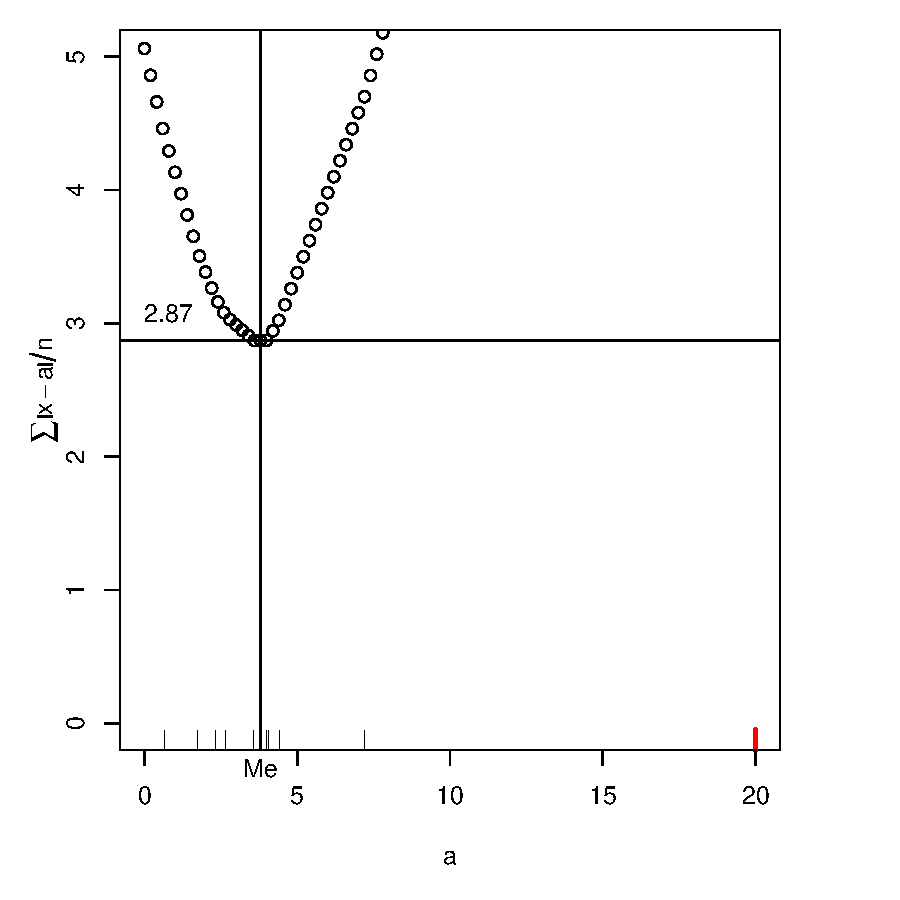
\includegraphics{./figs/mindevdev-004}
\end{center}


Minimum absolutnih in kvadratnih odklonov
\begin{center}
\begin{Schunk}
\begin{Sinput}
> showMinDeviation(what = c("median", "mean"), Xs = 20)
\end{Sinput}
\end{Schunk}
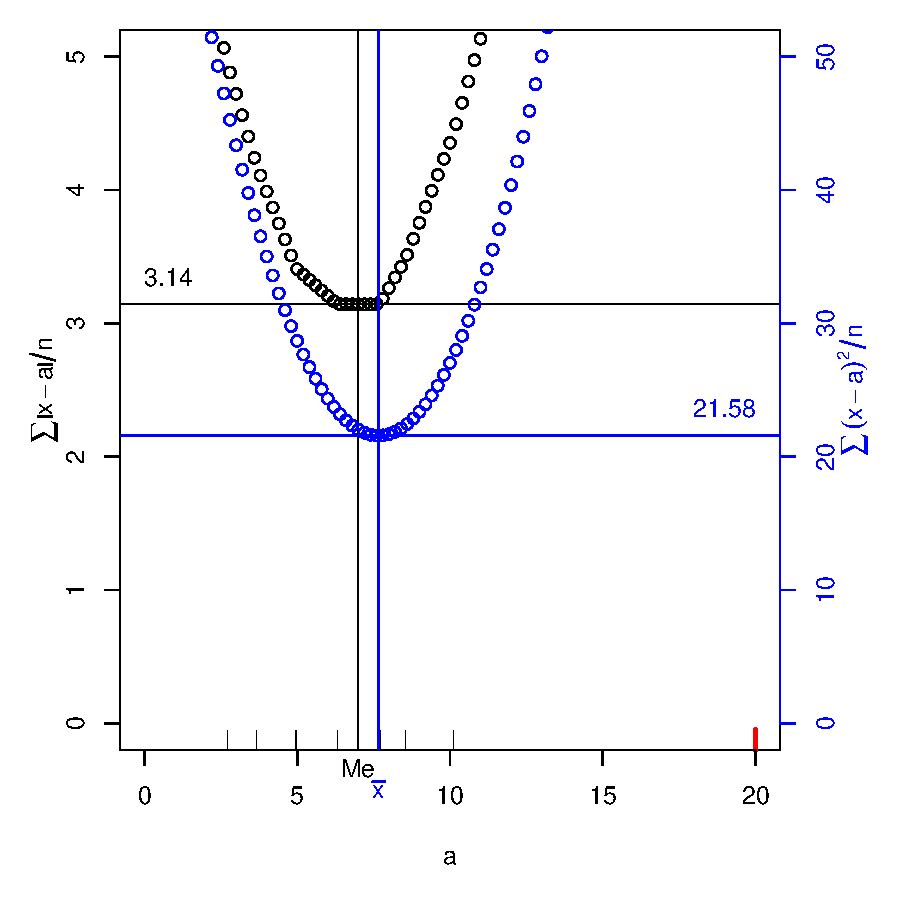
\includegraphics{./figs/mindevdev-005}
\end{center}
\clearpage
Minimumi pri mediani, povpre�ju in geometrijski sredini:
\begin{center}
\begin{Schunk}
\begin{Sinput}
> showMinDeviation(Xs = 20)
\end{Sinput}
\end{Schunk}
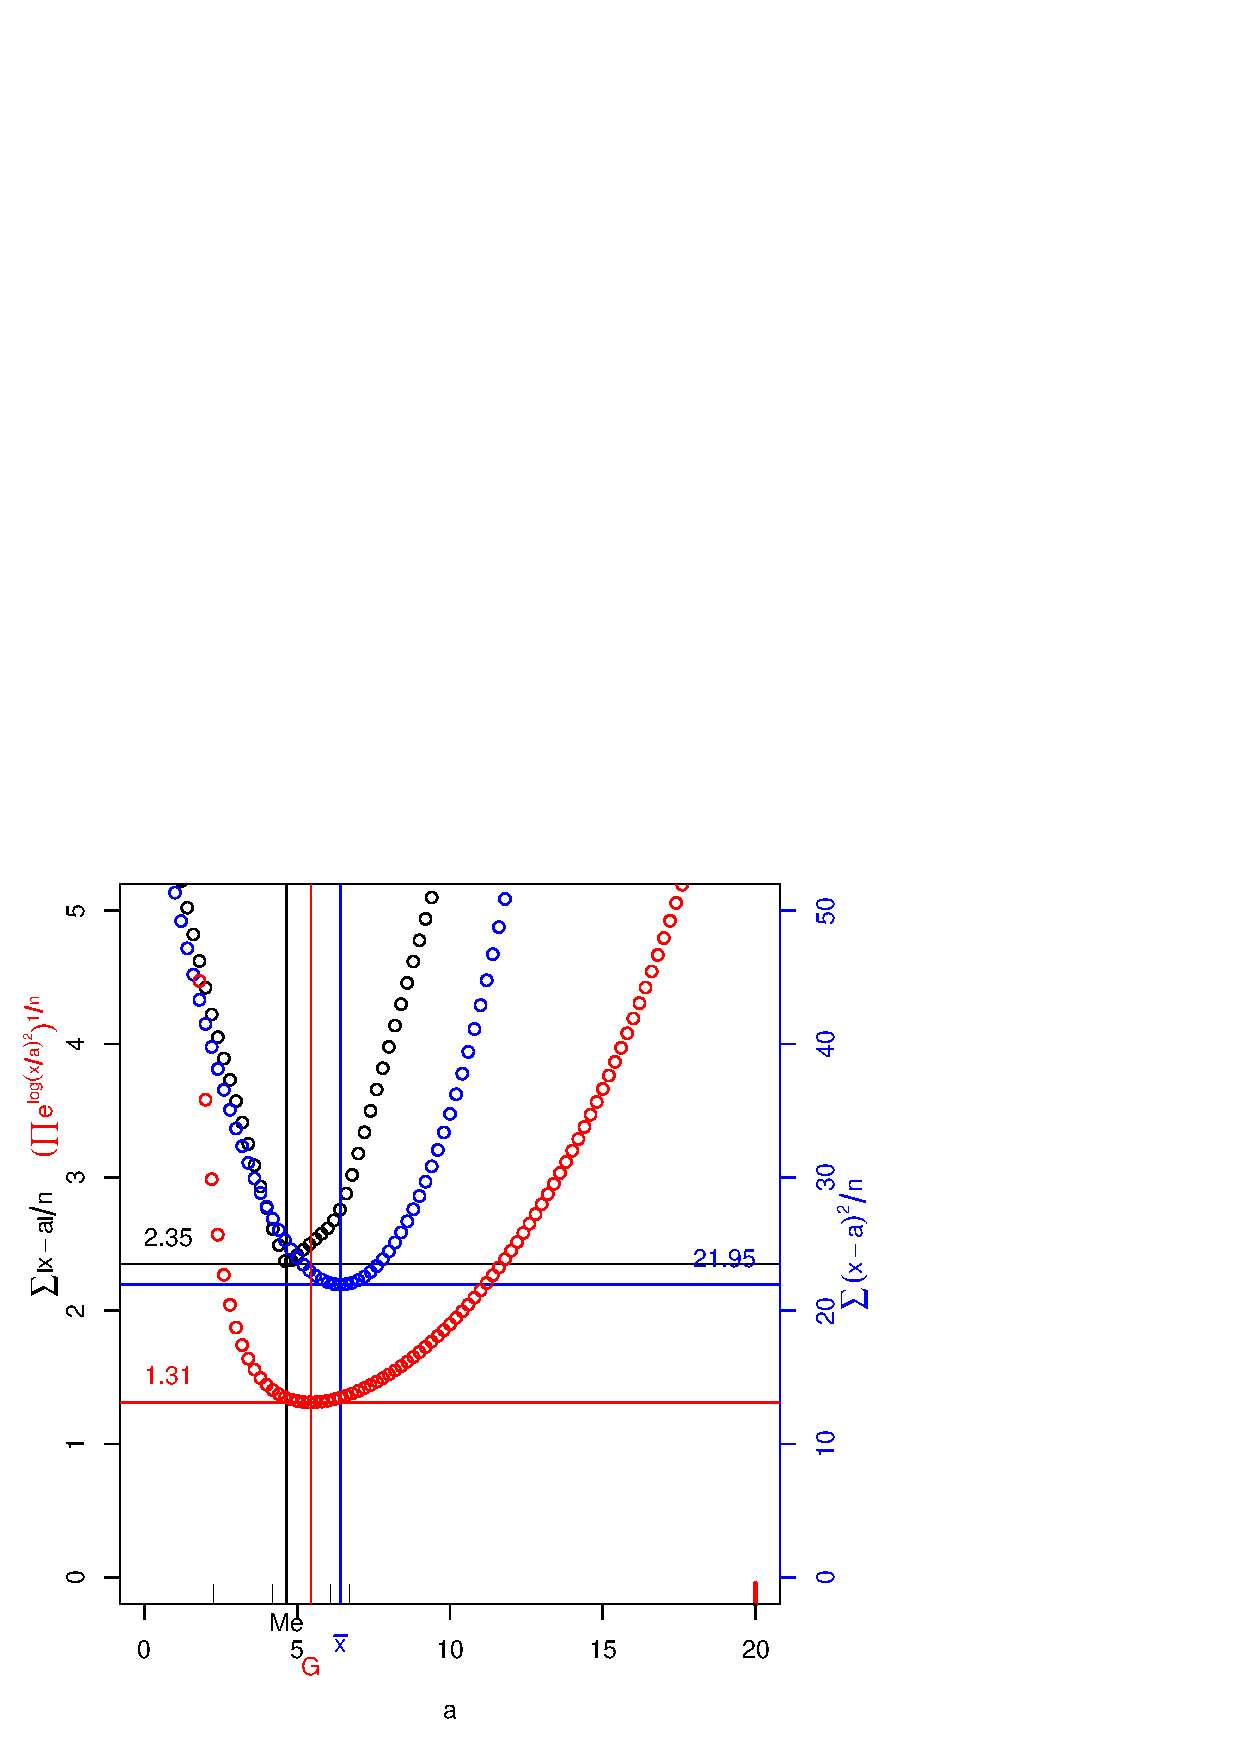
\includegraphics{./figs/mindevdev-006}
\end{center}


Za dinami�en prikaz prepi�ite funkcije iz razdelka \ref{s:fct} v \R pri �emer izpustite argument \code{Xs},
ki dolo�a kak�ne vrednosti naj ima eden od podatkov:

\begin{Schunk}
\begin{Sinput}
> showMinDeviation()
\end{Sinput}
\end{Schunk}
\clearpage
\section{Funkcije}\label{s:fct}
\subsection{\code{gmean}\\ Geometrijska sredina}
\begin{Schunk}
\begin{Sinput}
> gmean <- function(x, na.rm = TRUE) {
+     x <- x[!is.na(x)]
+     prod(x)^(1/length(x))
+ }
> gmean(c(1, 10, 100, NA))
\end{Sinput}
\begin{Soutput}
[1] 10
\end{Soutput}
\end{Schunk}

\subsection{\code{showMinDeviation}\\ Dinami�en prikaz ekstremov vsot odklonov}
\begin{Schunk}
\begin{Sinput}
> showMinDeviation <- function(x = rnorm(10, 5, 2), a = seq(0, 
+     20, 0.2), Xs = seq(0, max(a), 0.1), xlim = range(a), 
+     ylim = c(0, 5), what = c("median", "mean", "gmean"), 
+     cols = c("black", "blue", "red")) {
+     n <- length(x)
+     maxa <- max(a)
+     basey <- max(ylim)/15
+     vabs <- Vectorize(FUN = function(x, a) sum(abs(x - 
+         a))/length(x), "a")
+     vkv <- Vectorize(FUN = function(x, a) sum((x - a)^2)/length(x), 
+         "a")
+     pkvoc <- Vectorize(FUN = function(x, a) prod(exp(log(x/a)^2))^(1/length(x)), 
+         "a")
+     par(mar = c(5, 4, 1, 4))
+     for (X in Xs) {
+         x[n] <- X
+         plot(a, a, ylab = "", xlim = xlim, ylim = ylim, 
+             type = "n")
+         rug(x)
+         rug(x[n], col = "red", lwd = 3)
+         if (!is.na(pmatch("median", what))) {
+             col <- cols[1]
+             axis(1)
+             mtext(expression(sum(abs(x - a)/n)), 2, 2)
+             points(a, vabs(x, a), col = col)
+             abline(v = median(x), col = col)
+             MINa <- vabs(x, a = median(x))
+             abline(h = MINa, col = col)
+             text(0, MINa + 0.2, round(MINa, 2), xpd = TRUE, 
+                 adj = 0, col = col)
+             text(median(x), min(ylim) - basey, "Me", 
+                 xpd = TRUE, col = col)
+         }
+         if (!is.na(pmatch("mean", what))) {
+             col <- cols[2]
+             axis(4, col = col, at = axTicks(2), label = axTicks(2) * 
+                 10, col.axis = col)
+             mtext(expression(sum((x - a)^2)/n), 4, 2, 
+                 col = col)
+             points(a, vkv(x, a)/10, col = col)
+             abline(v = mean(x), col = col)
+             MINk <- vkv(x, a = mean(x))
+             abline(h = MINk/10, col = col)
+             text(maxa, MINk/10 + 0.2, round(MINk, 2), 
+                 xpd = TRUE, adj = 1, col = col)
+             text(mean(x), min(ylim) - basey * 1.5, expression(bar(x)), 
+                 xpd = TRUE, col = col)
+         }
+         if (!is.na(pmatch("gmean", what))) {
+             col <- cols[3]
+             points(a, pkvoc(x, a), col = col)
+             abline(v = gmean(x), col = col)
+             MINp <- pkvoc(x, a = gmean(x))
+             abline(h = MINp, col = col)
+             text(gmean(x), min(ylim) - basey * 2, "G", 
+                 xpd = TRUE, col = col)
+             text(0, MINp + 0.2, round(MINp, 2), xpd = TRUE, 
+                 adj = 0, col = col)
+             mtext(expression((prod(e^{
+                 log(x/a)^2
+             }))^{
+                 1/n
+             }), 2, 2, col = col, adj = 0.8)
+         }
+     }
+ }
> showMinDeviation()
\end{Sinput}
\end{Schunk}
\clearpage
\section{Minimum vsote absolutnih odklonov}

\newcommand{\sad}[1]{\sum_{#1} |x-a|}
\newcommand{\dsad}[1]{\frac{d \sad{#1}}{da}}

I��emo minimum vsote absolutnih odklonov
\begin{eqnarray*}
% \nonumber to remove numbering (before each equation)
  \sad{} &=& \sad{x\leq a}+\sad{x>a} \\
   &=& \sum_{x \leq a}(a-x) + \sum_{x > a}(x-a)
\end{eqnarray*}

Odvajajmo po $a$ in izena�imo z $0$:
\begin{eqnarray*}
% \nonumber to remove numbering (before each equation)
   \dsad{}&=& \frac{d \sum_{x \leq a}(a-x)}{da} +  \frac{d \sum_{x > a}(x-a)}{da}\\
   &=& \sum (+1) + \sum (-1) \\
   &=& n(x \leq a) - n(x> a)\\
   &=& 0
\end{eqnarray*}
kjer $n(\cdot)$ ozna�uje �tevilo vrednosti, ki ustrezajo pogoju v oklepaju.

Iz tega sledi, da dose�e izraz ni�lo za vsak $a$, za katerega je
 �tevilo vrednosti, ki so manj�e od $a$ enako �tevilu enot, ki so ve�je od $a$:
 $$n(x \leq a) = n(x> a)$$
 To pa je ravno lastnost mediane.
 
 Odvod je stopni�asta funkcija, ki se spremeni ko je $a$ enak kakemu podatku (slika \ref{f:ad}). Za $a$, ki so manj�i od mediane je odvod negativen, zato na tem delu z rasto�im $a$ vsota odklonov pada. Za $a$, ki so ve�ji od mediane pa je odvod pozitiven, zato za $a>Me$ vsota odklonov z rasto�im $a$ nara��a. Torej je ekstrem res minimum.



Zanimivo je, da je za sodo  �tevilo podatkov $n=2m$, odvod enak ni� za vse vrednosti $a$, ki so med srednjima podatkoma:

$$  x_m < a <x_{m+1} \Rightarrow D(a)=\dsad{}=0 $$


\vspace{1cm}
Za tiste, ki radi ri�emo :) je vse skupaj prikazano na sliki \ref{f:ad},
ki ka�e podatke (navpi�ne �rtice), vrednost odvoda $n(x \leq a) - n(x>a)$ (debele vodoravne �rte) in
vsoto odklonov (tanka �rta), ki je odsekoma linearna. Na sliki imamo 10 podatkov, tako da je dobro viden interval, na katerem je odvod enak ni�, vsota absolutnih odklonov pa ekstremno nizka in konstantna. 

\begin{center}

\begin{figure}
\begin{center}
  % Requires \usepackage{graphicx}
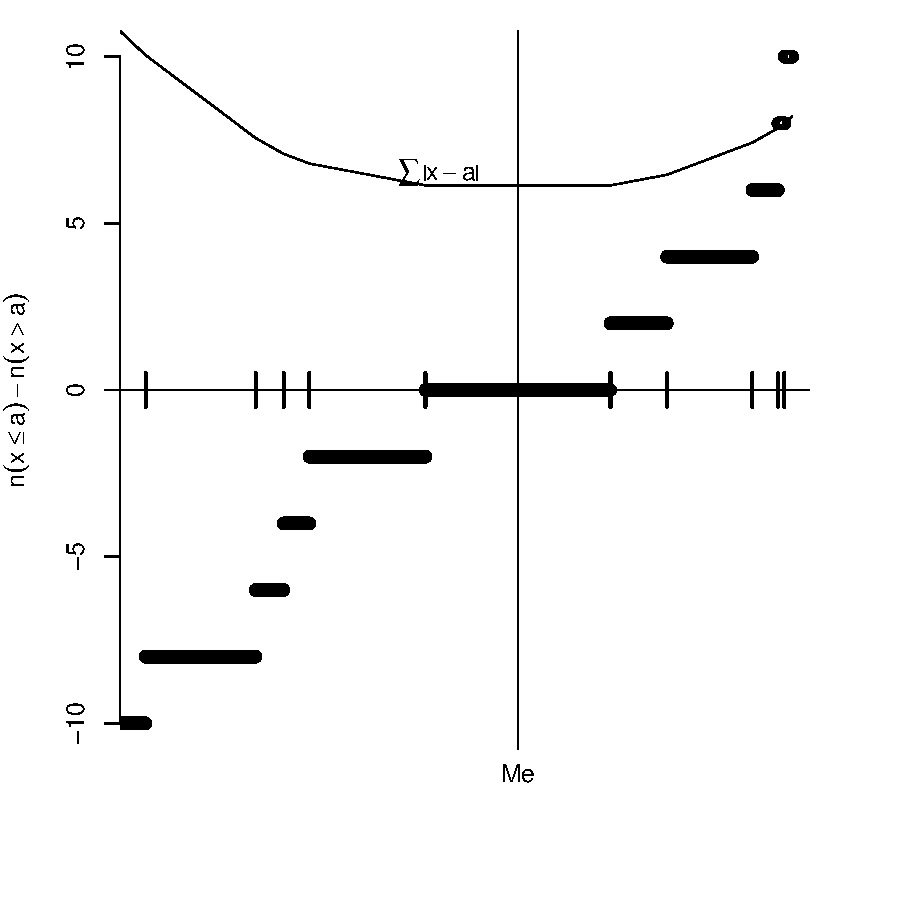
\includegraphics{./figs/mindevdev-minme}
  \caption{Odvod vsote absolutnih odklonov.}\label{f:ad}
\end{center}
\end{figure}
\end{center}


% ----------------------------------------------------------------
%\bibliographystyle{amsplain}
%\bibliography{}
\end{document}
% ----------------------------------------------------------------
